\documentclass[conference]{IEEEtran}
\IEEEoverridecommandlockouts
% The preceding line is only needed to identify funding in the first footnote. If that is unneeded, please comment it out.
\usepackage{cite}
\usepackage{amsmath,amssymb,amsfonts}
\usepackage{algorithmic}
\usepackage{graphicx}
\usepackage{textcomp}
\usepackage{xcolor}

\usepackage{url}
\usepackage{multirow}
\usepackage{tabularx}
\usepackage{enumitem}
\usepackage{booktabs}

\def\BibTeX{{\rm B\kern-.05em{\sc i\kern-.025em b}\kern-.08em
    T\kern-.1667em\lower.7ex\hbox{E}\kern-.125emX}}
\begin{document}

\title{Pseudo-Hierarchies for Robust Backbone Selection in Fine-Grained Image Recognition}

\author{Anonymous ICME submission}

\maketitle

\begin{abstract}

Fine-grained image recognition (FGIR) involves distinguishing visually similar subcategories that are often organized in hierarchical structures. While prior work has leveraged hierarchies for FGIR, the role of the backbone and its interaction with hierarchical supervision and hyperparameter robustness remains underexplored. In this work, we benchmark 21 pretrained convolutional and transformer models under both fine-tuned and frozen settings, highlighting backbone selection as a critical factor in hierarchical FGIR. We then study the effect of hierarchical supervision on hyperparameter robustness, introducing the Accuracy Deviation-to-Average (ADA) ratio to quantify sensitivity to hyperparameter choices. Our results demonstrate that hierarchical structure consistently improves robustness. Finally, to alleviate reliance on manually annotated hierarchies, we explore pseudo-hierarchies constructed via clustering, and show that systematically generated hierarchies can achieve comparable robustness gains. Our findings provide practical guidance for robust backbone selection and hierarchical design in FGIR.

\end{abstract}

\begin{IEEEkeywords}
Fine-Grained Object Categorization, Hierarchical Classification, Pseudo-Labels
\end{IEEEkeywords}

\section{Introduction}
\label{sec:intro}

Fine-grained image recognition (FGIR) aims to distinguish between visually similar subcategories within a broader class. Although these categories are often organized hierarchically, early FGIR methods treat labels as flat categories \cite{zhang_part-based_2014, zheng_learning_2017}, ignoring semantic structure and resulting in suboptimal performance \cite{chen_fine-grained_2018}. Hierarchical FGIR addresses this by leveraging multi-level semantic relationships, using coarse-level predictions to guide fine-grained classification \cite{chen_fine-grained_2018, chang_your_2021}. However, these methods overlook a fundamental factor: the backbone.

% This limits their ability to exploit hierarchical cues, resulting in suboptimal performance \cite{chen_fine-grained_2018}. 

% Several approaches have explored this direction, such as granularity specific classifiers \cite{chang_your_2021} and hierarchically discriminative loss functions \cite{chen_fine-grained_2018}. 

The backbone impact has been previously studied for general image classification \cite{kornblith_better_2019, goldblum_battle_2023, jeevan_which_2025} and weakly supervised FGIR \cite{ye_image_2024}, but its role in hierarchical FGIR is underexplored. Most hierarchical FGIR methods continue to rely on a narrow set of backbones \cite{wang_multiple_2015, cerri_reduction_2016, chen_fine-grained_2018, chang_your_2021, chen_label_2022, chen_hierarchically_2024}, leaving open the question: \textbf{to what extent does the backbone influence FGIR performance in the presence of hierarchical labels?}

Furthermore, the selection and sensitivity to hyperparameters of FGIR models has been neglected. It is often assumed that hyperparameters tuned on one dataset can generalize to similar targets \cite{ngiam_domain_2018}. However, common defaults for learning rate, weight decay, and other optimization parameters produce unreliable results after fine-tuning \cite{li_rethinking_2020}. Hyperparameter searches are computationally expensive and contribute significantly to the carbon footprint of deep learning pipelines \cite{strubell_energy_2019, lacoste_quantifying_2019}, making robustness to hyperparameter variation important for stable and dependable model deployment.

In this work, we conduct \textbf{the first study on robust backbone selection for hierarchical FGIR}. We benchmark a wide range of convolutional and transformer-based models across multiple datasets and hyperparameters, showing that backbone choice has a large impact, from state-of-the-art performance (91\% wAP on CUB for ViT \cite{dosovitskiy_image_2021}), to poor results (80\% wAP on CUB for CLIP \cite{cherti_reproducible_2023}), as shown in Figure \ref{fig_four_plot}. 

To measure the robustness to hyperparameter choices of a backbone, we introduce the \textbf{Accuracy Deviation-to-Average (ADA) ratio}. ADA computes the ratio of standard deviation to average performance across different hyperparameters as a robustness metric; a lower ADA indicates lower variance and higher mean across different hyperparameters. Through ADA we observe that many backbones are sensitive to hyperparameters, specially transformer-based models. Importantly, we find that introducing hierarchical supervision consistently reduces ADA across architectures and datasets (see Table \ref{tab:baseline_vs_hierarchy}). Hierarchical labels lowers sensitivity to hyperparameters and narrows the robustness gap between backbones, in some cases reducing ADA by more than half compared to the baseline without hierarchical labels.

However, this robustness gain relies on human-annotated hierarchies, which are time-consuming and expensive to construct; limiting the practical adoption of hierarchical FGIR. Since hierarchies increases hyperparameter robustness, we ask the question: \textbf{can robustness be achieved without a manually constructed hierarchy?} We propose a \textbf{pseudo-hierarchy} strategy that builds hierarchical structure systematically from feature representations and existing fine-grained labels. Our approach constructs hierarchies in a bottom-up manner by grouping fine-level classes into coarser categories using bipartite matching. Through experiments, we show that pseudo-hierarchies provide robustness improvements comparable to human-annotated hierarchies without requiring annotation costs.

Our study offers three main contributions: 
\begin{enumerate} [topsep=3pt, itemsep=2pt, parsep=1pt]
    \item We study 21 pretrained backbones (11 CNNs, 10 ViTs) in determining hierarchical FGIR performance. The right choice of backbone can \textbf{change wAP by up to 11\%}.
    \item We evaluate hierarchical supervision across backbones and datasets. Hierarchy consistently improves robustness, reducing ADA up to \textbf{75\%} compared to FGIR baselines.
    \item We propose Bipartite Pseudo-Hierarchy (BPH), a novel pseudo-hierarchy construction that alleviates the cost of manual annotation, and show that pseudo-hierarchies can improve robustness, reducing ADA by up to \textbf{50\%}.
\end{enumerate}

\section{Related Works}
\subsection{Fine-Grained Image Recognition(FGIR)}
Early FGIR methods relied on part annotations or bounding boxes to guide localization \cite{zhang_part-based_2014}. While effective, these methods are difficult to scale due to the cost of annotations.  Later works leveraged image-level labels with attention mechanisms, such as MA-CNN \cite{zheng_learning_2017}, which learned part-aware features without extra supervision. However, these models ignored class hierarchies, limiting their ability to capture semantic structure and generalize across categories.

\subsection{Hierarchical Fine-Grained Image Recognition}
To address these limitations, hierarchical FGIR methods introduce multi-level prediction heads and hierarchy-aware losses. One of the first works, Multi-Granularity Descriptor (MGD) \cite{wang_multiple_2015}, used weakly supervised taxonomic descriptors. This was followed by methods like Hierarchical Semantic Embedding (HSE) \cite{chen_fine-grained_2018} and granularity-specific classifiers \cite{chang_your_2021}, which introduced hierarchy-aware loss functions and multi-level prediction heads. Though effective, these methods still struggle with class ambiguity within coarse groups and rely on a narrow set of backbone architectures.

\subsection{Backbone effect on FGIR}
Recent works have explored the impact of backbone architectures on transfer learning and FGIR. Kornblith et al. \cite{kornblith_better_2019} analyzed whether higher ImageNet accuracy leads to better downstream performance, while Goldblum et al. \cite{goldblum_battle_2023} and Jeevan et al. \cite{jeevan_which_2025} focused on backbone impact in general image classification. Ye et al. \cite{ye_image_2024} investigated backbones for weakly supervised FGIR. However, these works neglect the impact of hierarchical labels and robustness to hyperparameter choices for the backbones. Our work systematically investigates how backbone choice interacts with hierarchy, using the ADA ratio to evaluate robustness across hyperparameters, offering new insights for hierarchical FGIR.

\subsection{Pseudo-Hierarchies in Image Classification}
Pseudo-hierarchies are widely used in general image classification, such as anomaly detection \cite{wang_hierarchical_2022} and satelite imagery \cite{liu_clustering-based_2025}. They are typically built top-down and using unsupervised hierarchical clustering. In FGIR, pseudo-hierarchies have also been explored \cite{znalezniak_contrastive_2023}, with many employing bottom-up hierarchies. Our approach constructs hierarchies using feature representations from pretrained models and existing fine labels to merge categories into coarser groups, leveraging pseudo-hierarchies while adapting them to the fine-grained scenario.

\begin{figure}[ht]
    \centering
    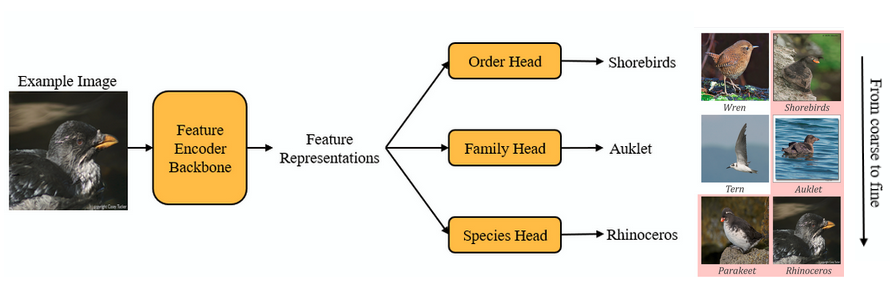
\includegraphics[width=1\linewidth]{figures/imgs/architecture.png}
    \caption{Overview of the image classification pipeline used in our experiments.}
    \label{fig:architecture}
\end{figure}

\section{Experiment Setup}
\subsection{Architecture Overview}

Our architecture, shown in Figure \ref{fig:architecture}, follows the hierarchical pipeline of Chang et al. \cite{chang_your_2021}, where an image is processed by a shared feature encoder (backbone), followed by classifier heads for each taxonomy level. Each level targets labels from coarse to fine. We evaluated different backbones spanning two types, 10 Transformer (ViT-B) and 11 CNN (ResNet50). The 21 models are shown in Table \ref{tab:ada_ratio}.

Three datasets are used: \textbf{FGVC Aircraft} \cite{maji_fine-grained_2013}, \textbf{CUB-200-2011} \cite{wah_caltech-ucsd_2011}, and \textbf{Stanford Cars} \cite{krause_collecting_nodate}.Hierarchies are constructed from Wikipedia class taxonomies following Chang et al. \cite{chang_your_2021}.

To assess model effectiveness in hierarchical FGIR, we measure several evaluation metrics measuring individual level, cross-level accuracy and robustness:
\begin{itemize}
    \item \textbf{Per-level accuracy}. The Top-1 classification accuracy of each level in the hierarchy. There are \textbf{3 hierarchical levels} at most, these are denoted by \textbf{L3, L2, L1, from coarsest to finest}.

    \item \textbf{Weighted Average Precision (wAP).}  
    to address class imbalance, wAP weights per-class accuracy by sample count
    wAP is defined as:
    \[
    wAP = \frac{1}{N} \sum_{k=1}^{K} n_k \cdot \text{Acc}_k
    \]
    where $K$ is the number of classes, $n_k$ is the number of samples in class $k$, $\text{Acc}_k$ is the accuracy for class $k$, and $N = \sum_{k=1}^{K} n_k$ is the total number of samples.
    
    \item \textbf{ADA ratio}. 
    inspired by the coefficient of variation \cite{brown_applied_1998}, this metric balances accuracy and robustness by measuring the ratio of standard deviation to mean accuracy across multiple runs.
    ADA ratio is defined as:
    \[
    ADA\ ratio = \frac{\sigma}{\mu} \times 100\% 
    \]
    where $\mu$ denotes the mean accuracy and $\sigma$ the standard deviation across evaluation runs. Specifically, on Table \ref{tab:ada_ratio} we computed the ADA ratio across different hyperparameters and datasets. Lower ADA ratio indicates a model achieves both high mean accuracy and low deviation, desirable characteristics in practical deployments. 
\end{itemize}

We compare 2 different training settings: \textbf{fine-tuning (FT)}, where all parameters are updated, and \textbf{frozen backbone (FZ)}, where only the classifier head is trained. All models are trained for 200 epochs with a batch size of 8. To study the impact of hyperparameters, we use two optimizers (SGD and AdamW) across 10 learning rates, SGD (0.3–0.003) with weight decay 0, and AdamW (0.005–0.000005) with weight decay 0.05. We employ cosine learning rate scheduler and mixed precision. During training we employ standard data augmentation (resize to 550×550, random crop to 448×448, horizontal flip). Center cropping is used during inference.

\begin{table}[!htb]
    \centering
    % \small
    \caption{ADA Ratio across different hyperparameters and datasets. Lower is better. Best and second best are \textbf{bold faced} and \underline{underlined}, respectively.}
    \label{tab:ada_ratio}
    \begin{tabularx}{\linewidth}{p{2.9cm}p{1.75cm}XX}
        \toprule
        Method & Fine-tuned & Frozen & Average \\
        \midrule
        \multicolumn{4}{>{\raggedright\arraybackslash}p{\linewidth}}{\textbf{ResNet50 models (CNN-based)}} \\
        \multicolumn{4}{>{\raggedright\arraybackslash}p{\linewidth}}{\textit{Fully-Supervised models}} \\
        RN TV1\cite{he_deep_2015} & 2.44 & 2.98 & 2.71 \\
        RN TV2\cite{he_deep_2015} & 1.39 & 1.24 & 1.31 \\
        RN Gluon\cite{he_bag_2018} & 2.61 & 1.41 & 2.01 \\
        RN IN21k-P\cite{ridnik_imagenet-21k_2021} & 1.54 & 1.04 & \underline{1.29} \\
        RN A1\cite{wightman_resnet_2021} & 2.42 & 0.96 & 1.69 \\
        \multicolumn{4}{>{\raggedright\arraybackslash}p{\linewidth}}{\textit{Semi-Supervised models}} \\
        RN IG1b\cite{yalniz_billion-scale_2019} & 4.28 & 1.18 & 2.73 \\
        RN YFCC100m\cite{yalniz_billion-scale_2019} & 3.53 & 1.5 & 2.51 \\
        \multicolumn{4}{>{\raggedright\arraybackslash}p{\linewidth}}{\textit{Self-Supervised models (Discriminative)}} \\
        RN SupCon\cite{khosla_supervised_2021} & 3.24 & 1.37 & 2.31 \\
        RN SwAV\cite{caron_unsupervised_2021} & \underline{1.33} & 1.46 & 1.39 \\
        RN MoCo v3\cite{chen_empirical_2021} & \textbf{1.18} & 1.32 & \textbf{1.25} \\
        \multicolumn{4}{>{\raggedright\arraybackslash}p{\linewidth}}{\textit{Self-Supervised models (Generative)}} \\
        RN SparK\cite{tian_designing_2023} & 5.67 & 3.92 & 4.8 \\
        \midrule
        \multicolumn{4}{>{\raggedright\arraybackslash}p{\linewidth}}{\textbf{ViT-B models (Transformer-based)}} \\
        \multicolumn{4}{>{\raggedright\arraybackslash}p{\linewidth}}{\textit{Fully-Supervised models}} \\
        ViT\cite{dosovitskiy_image_2021} & 11.35 & 1.01 & 6.18 \\
        DeiT\cite{touvron_training_2021} & 12.79 & 0.77 & 6.78 \\
        ViT IN21k-P\cite{ridnik_imagenet-21k_2021} & 17.43 & 1.98 & 9.7 \\
        DeiT 3 (IN1k)\cite{touvron_deit_2022} & 13.55 & 1.06 & 7.31 \\
        DeiT 3 (IN21k)\cite{touvron_deit_2022} & 18.42 & \textbf{0.59} & 9.51 \\
        \multicolumn{4}{>{\raggedright\arraybackslash}p{\linewidth}}{\textit{Self-Supervised models (Discriminative)}} \\
        ViT MoCo v3\cite{chen_empirical_2021} & 20.13 & 1.24 & 10.68 \\
        ViT DINO\cite{caron_emerging_2021} & 42.36 & 0.96 & 21.66 \\
        ViT CLIP\cite{cherti_reproducible_2023} & 52.52 & \underline{0.63} & 26.58 \\
        ViT SigLIP v2\cite{tschannen_siglip_2025} & 31.34 & 2.1 & 16.72 \\
        \multicolumn{4}{>{\raggedright\arraybackslash}p{\linewidth}}{\textit{Self-Supervised models (Generative)}} \\
        ViT MAE\cite{he_masked_2021} & 28.2 & 4.44 & 16.32 \\
        \bottomrule
    \end{tabularx}
\end{table}

\begin{figure*}[!htb]
    \centering
    \begin{minipage}{0.41\linewidth}
        \centering
        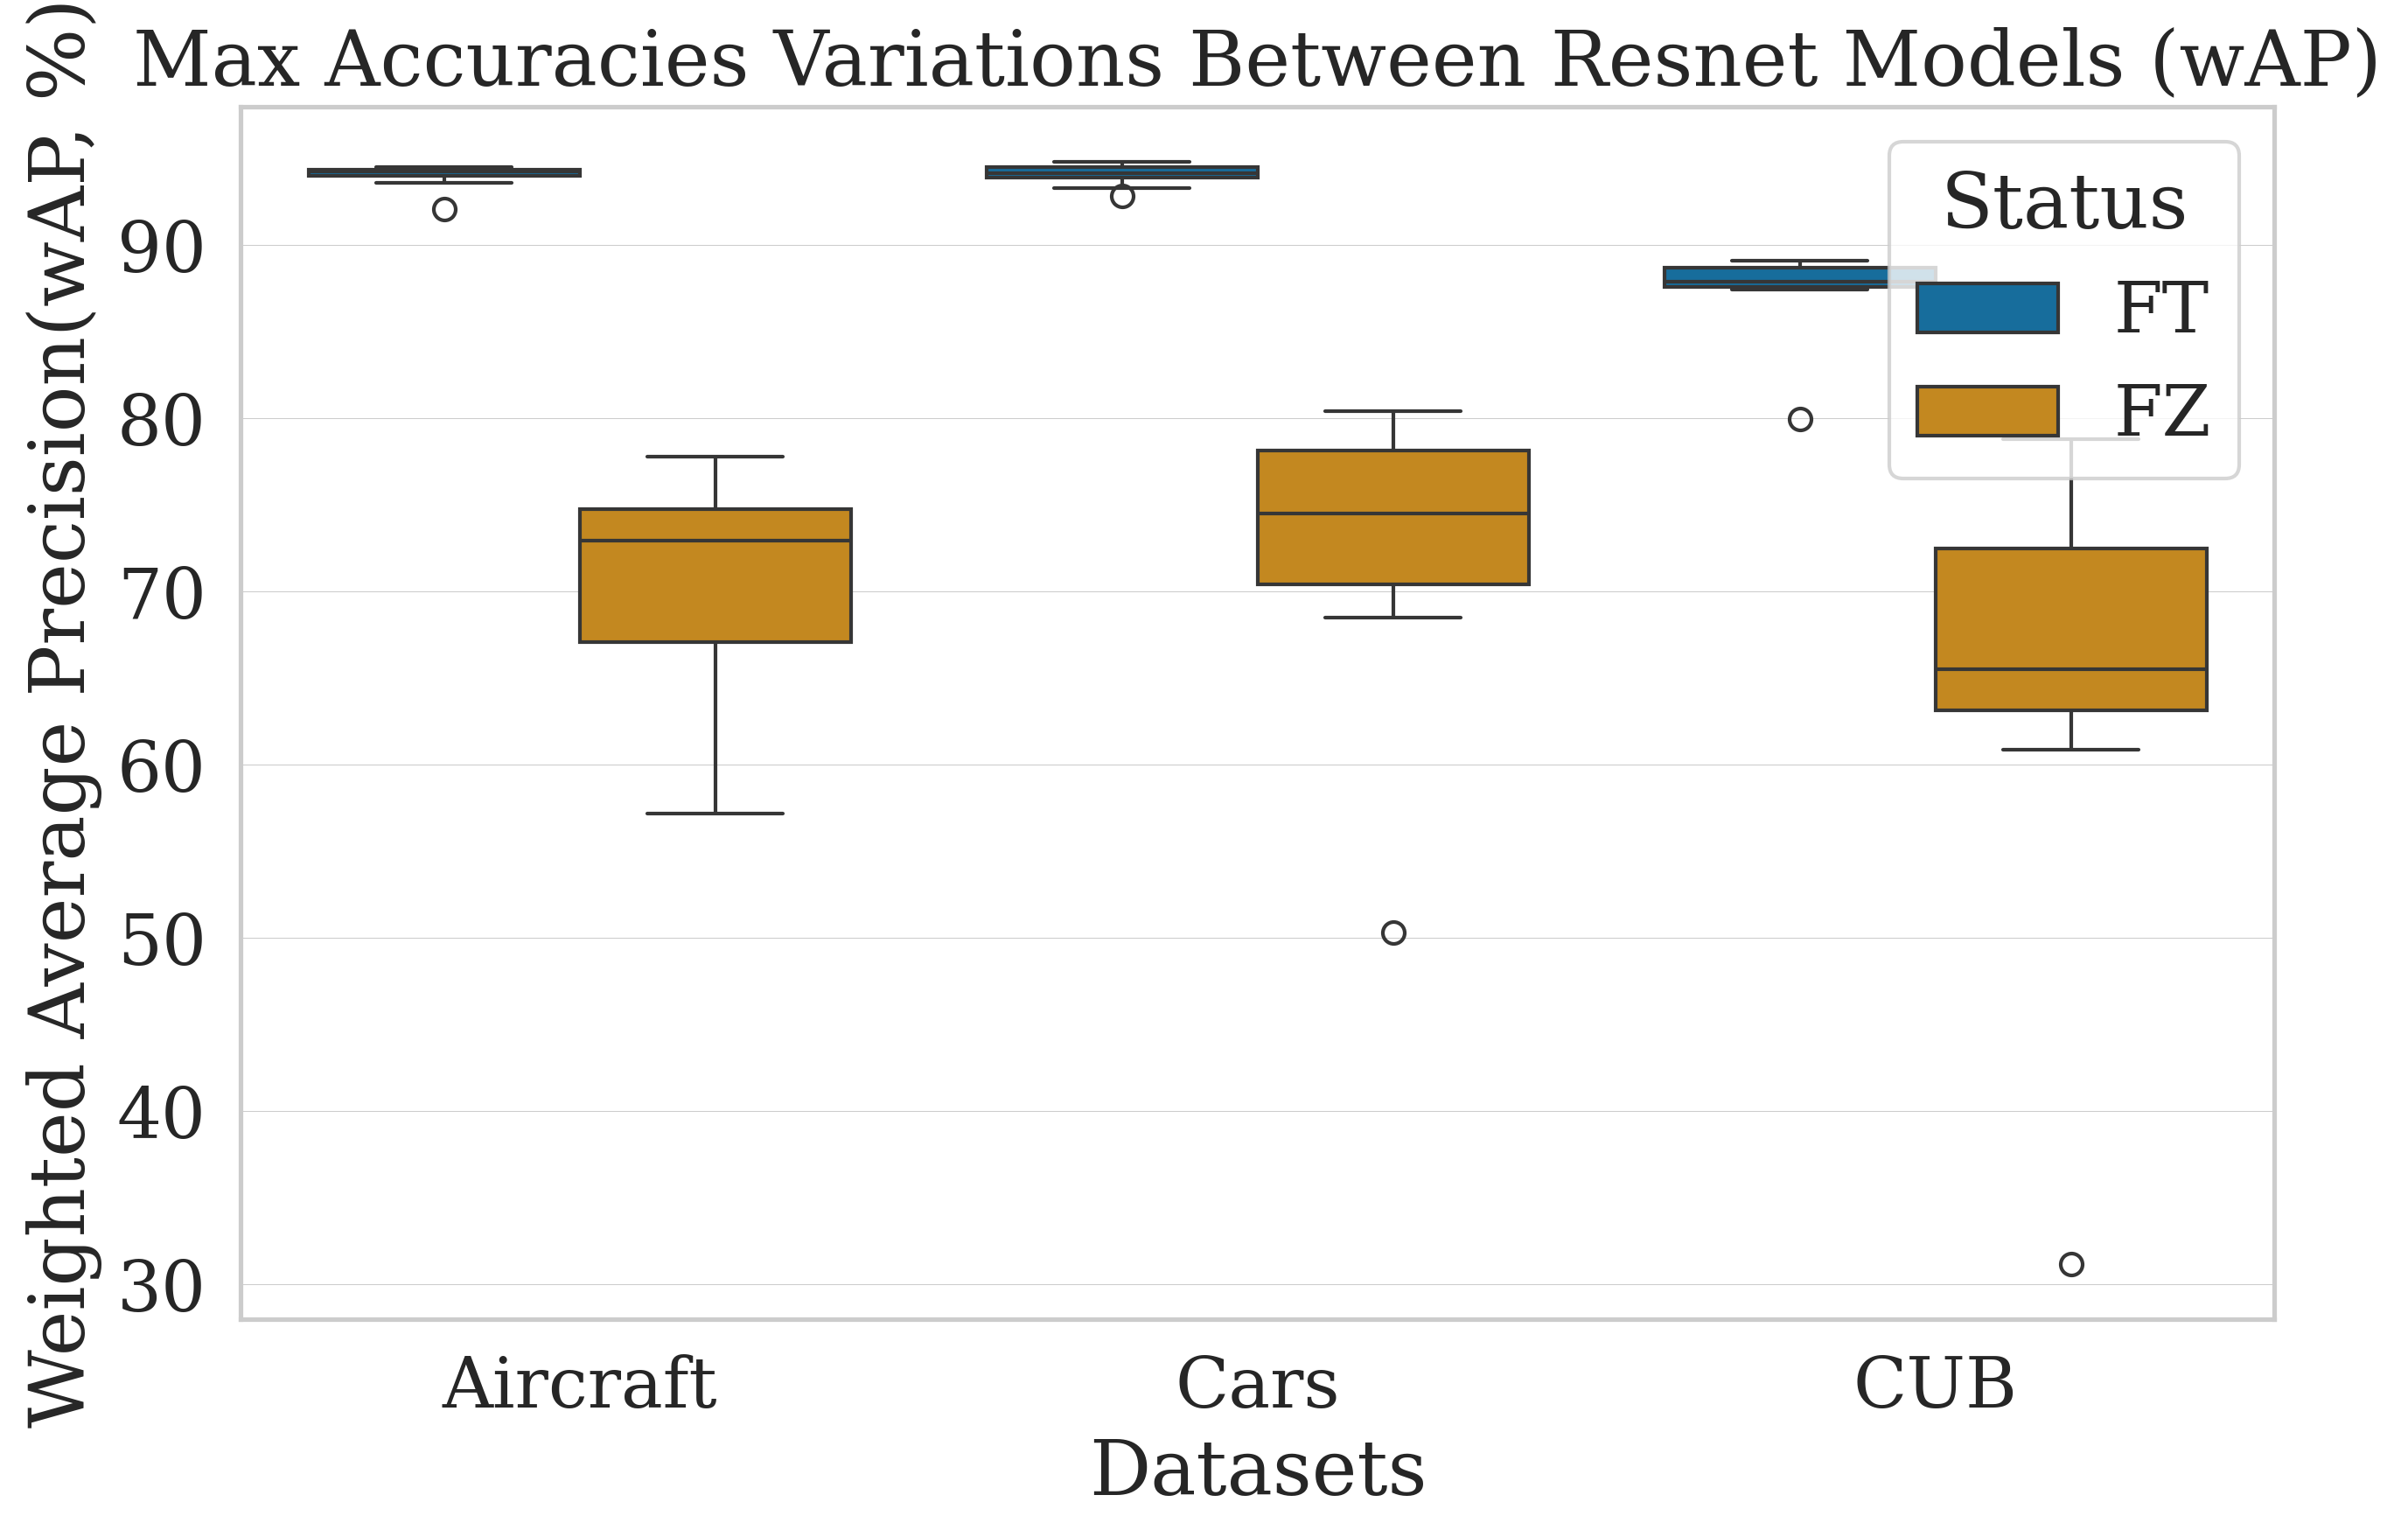
\includegraphics[width=\linewidth]{figures/imgs/performance_left.png}
        \label{fig_resnet_perf}
    \end{minipage}
    \hspace{0.01\linewidth} % Reduce spacing
    \begin{minipage}{0.40\linewidth}
        \centering
        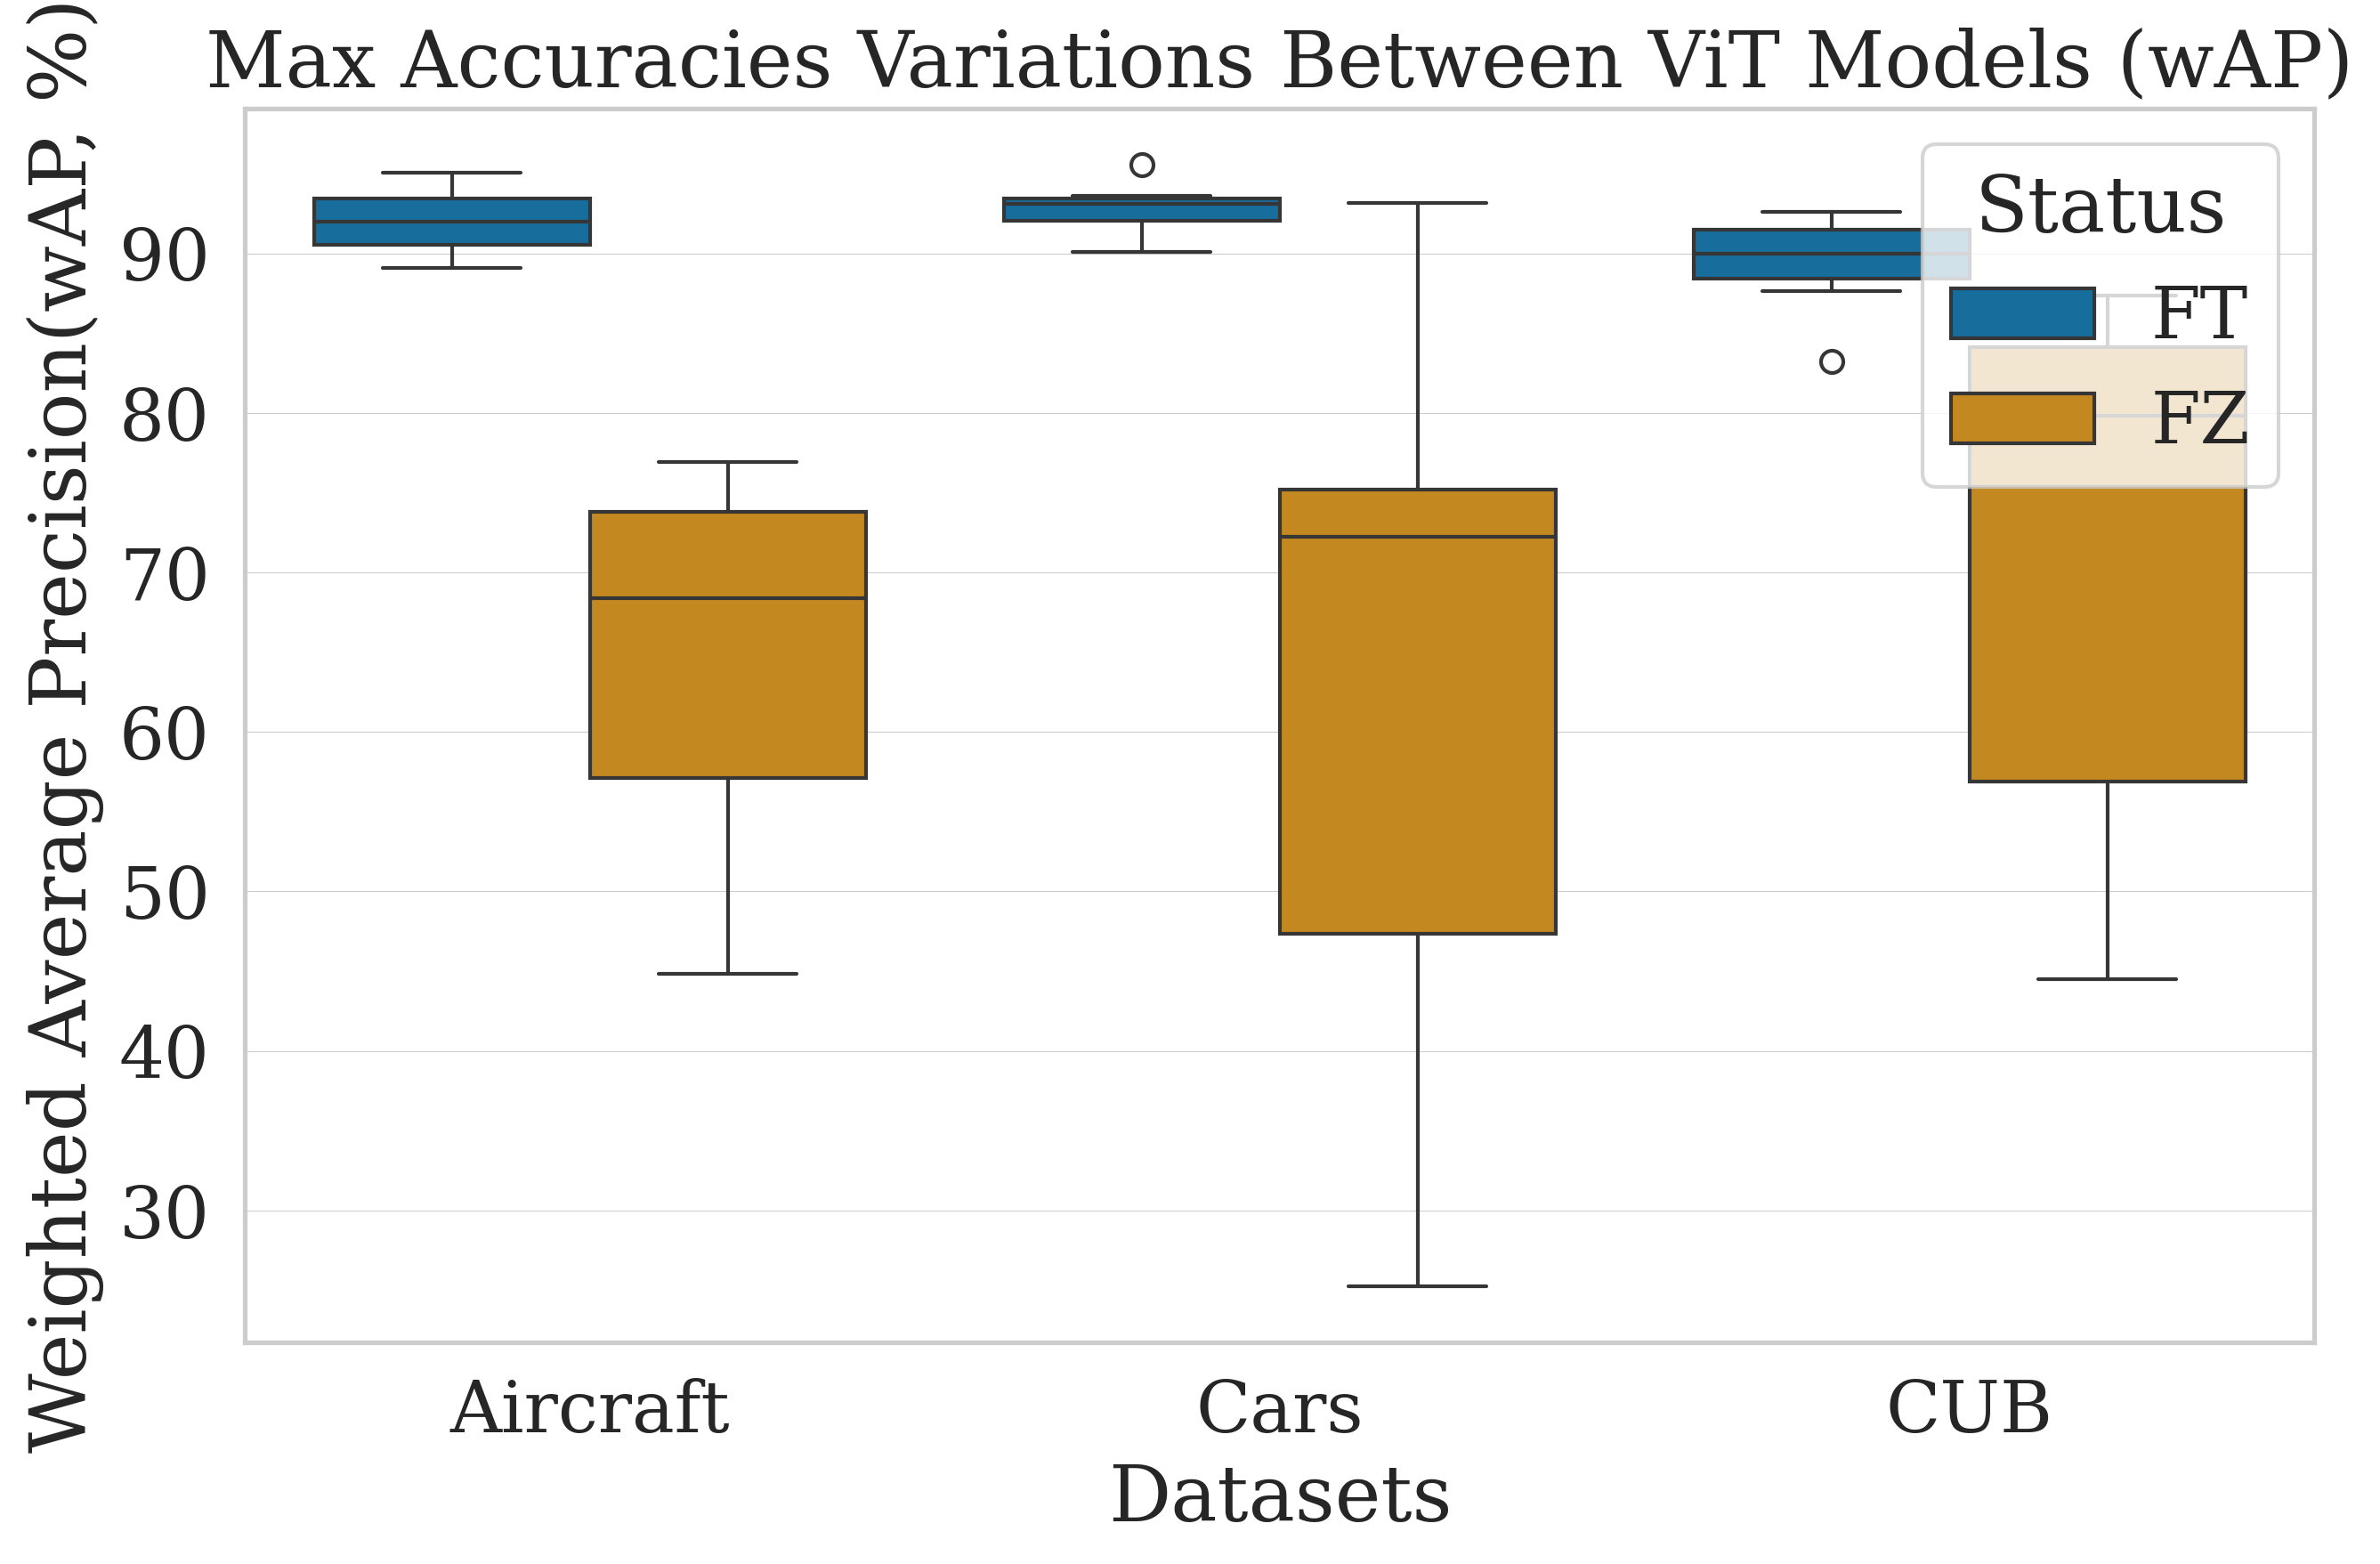
\includegraphics[width=\linewidth]{figures/imgs/performance_right.png}
        \label{fig_vit_perf}
    \end{minipage}
    \vspace{-0.55cm}
    \caption{Performance variability across backbone types and training modes. We compare fine-tuned (FT) and frozen (FZ) variants of ResNet (left) and ViT (right) models across hierarchical FGIR benchmarks.}
    \label{fig_performance}
\end{figure*}


\subsection{Pseudo-Hierarchy Setup}
To alleviate the costs of manually annotated hierarchies we propose Bipartite Pseudo-Hierarchy (BPH), a method to systematically construct coarse-level pseudo-hierarchies from fine-grained labels. First, we extract feature tensors from the last BatchNorm layer of ResNet models and the last LayerNorm layer of ViT models; fine-level centroids are computed from these feature tensors. These are grouped into coarse-level clusters using bipartite matching via Hungarian algorithm \cite{kuhn_hungarian_1955}, forming a hierarchy of super-classes. Each sample is assigned to the cluster of its fine-level centroid. 

We evaluate the effect of pseudo-hierarchy using the ResNet IG1b \cite{yalniz_billion-scale_2019} model, which is the most unstable ResNet variant in our experiments. Experiments are conducted on the Aircraft and CUB datasets with 2 settings:

\begin{itemize} [topsep=3pt, itemsep=2pt, parsep=1pt]
    \item Pseudo-hierarchy generated using the same model as the evaluation model (ResNet IG1b)
    \item Pseudo-hierarchy generated using a stronger model different from the evaluation model (ViT SigLipv2)
\end{itemize}

We construct a 2-level pseudo-hierarchy with 6 ratios of coarse-level to fine-level labels: 10, 20, 30, 40, 50 and 70. For example, 10 represents that there are 10\% of coarse-level labels to fine-grained labels (e.g., 10 coarse-level for 100 fine-level classes).

\section{Results}
\subsection{Impact of Backbone and Pretraining on FGIR}
\subsubsection{Backbone Choice Drives Performance}
Fig. \ref{fig_performance} highlights how backbone selection alone can lead to vastly different outcomes. Among ResNets, MoCoV3 performs best (94\% wAP on Aircraft), while the worst performing one, Spark obtains 92\% wAP. ViT models show larger performance variance: SigLIP-v2 excels on Aircraft (94\%) and Cars (95\%), while original ViT excels CUB (91\%). In contrast, DINO performs worst with 87\% on Aircraft and 89\% on Cars. These findings shows that backbone selection, especially for ViTs, can lead to \textbf{state-of-the-art performance or degraded results}.

\begin{figure}[ht]
    \centering
    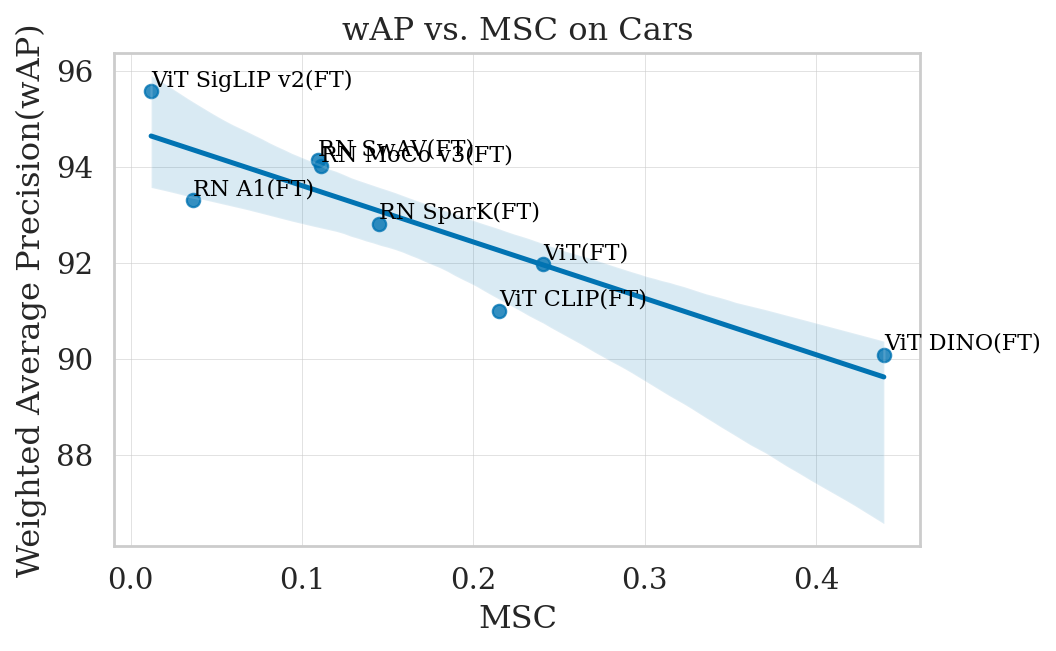
\includegraphics[width=0.85\linewidth]{figures/imgs/example_plot.png}
    \caption{Plot showing wAP vs. MSC for the Top-2 and Worst-2 Resnet and ViT fine-tuned models. ViT SigLiP is far away from the rest of the ViT.} 
    \label{fig_example_metric}
\end{figure}

\subsubsection{Resnet models do better on machines, but ViT models
do better on animals}
\label{sec:dataset_differences}
In Fig. \ref{fig_performance} and Fig. \ref{fig_four_plot} \textbf{ResNet models} generally \textbf{perform better} on \textbf{Aircraft and Cars}, while \textbf{ViTs do better} on \textbf{CUB}. This aligns with Ye et al.\cite{ye_image_2024}, which suggests that \textbf{objects with more dynamic shapes} (e.g. animals) \textbf{benefit} more from the \textbf{self-attention mechanism} in transformers. In contrast, \textbf{objects with more static shapes} (e.g. machines) \textbf{benefit} from the \textbf{inductive biases} in CNNs. Also, ImageNet contains a substantial number of bird-related images, which may have contributed to a performance boost for ViT models on the CUB dataset.

However, we observe \textbf{an exception}: \textbf{SigLIPv2}, a ViT model, achieves \textbf{better performance} on \textbf{Aircraft and Cars} than the \textbf{best ResNet model}, challenging this observation. To explain this, we employ \textbf{Mean Silhouette Coefficient (MSC)} \cite{rousseeuw_silhouettes_1987}, which quantifies the quality of feature clustering based on inter-class separation\cite{islam_broad_2021} and intra-class variance\cite{islam_broad_2021}. Higher values indicate well-separated and compact class clusters, while lower values imply more ambiguous features. We plot the Top-2 and Worst-2 wAP vs MSC for clarity, as observed in \ref{fig_example_metric}, SigLIP obtains lower MSC compared to other ViTs, suggesting tighter and less distinct feature representations. We also observed that ResNets obtains lower MSC than ViTs, while SigLiP obtains lower values than ResNets. This indicate that \textbf{performance stems from learned representations during pretraining rather than only architectural biases}.


\begin{table}[t]
\centering
\caption{ADA ratio across hyperparameters comparing baseline without hierarchical labels vs model with hierarchical labels. Lower is better.}
\label{tab:baseline_vs_hierarchy}
\begin{tabularx}{\linewidth}{p{1.8615cm}XXXXXX}
\toprule
% \multirow{2}{*}{Method} & \multicolumn{2}{c}{Aircraft} & \multicolumn{2}{c}{Cars} & \multicolumn{2}{c}{CUB} \\
Method & \multicolumn{2}{c}{Aircraft} & \multicolumn{2}{c}{Cars} & \multicolumn{2}{c}{CUB} \\
\cmidrule(lr){2-3} \cmidrule(lr){4-5} \cmidrule(lr){6-7}
Hier. Labels & - & \checkmark & - & \checkmark & - & \checkmark \\
\midrule
RN YFCC100m & 2.16 & 1.59 & 5.64 & 2.51 & 7.60 & 6.51 \\
RN IG1b     & 3.08 & 1.73 & 7.51 & 0.70 & 8.67 & 6.19 \\
RN Gluon    & 1.68 & 1.47 & 3.03 & 2.51 & 5.46 & 3.85 \\
RN TV1      & 1.47 & 1.30 & 3.12 & 2.39 & 5.95 & 3.63 \\
RN TV2      & 1.31 & 1.12 & 1.47 & 0.71 & 4.07 & 2.33 \\
\midrule
ViT              & 25.00 & 6.25 & 44.30 & 7.62 & 21.63 & 20.19 \\
DeiT             & 26.14 & 4.29 & 29.88 & 15.24 & 17.03 & 18.21 \\
ViT IN21k-P      & 22.73 & 7.94 & 40.56 & 27.39 & 28.29 & 16.95 \\
DeiT 3 (IN1k)    & 30.38 & 6.75 & 35.88 & 19.93 & 24.46 & 12.93 \\
DeiT 3 (IN21k)   & 29.01 & 11.82 & 48.65 & 20.03 & 27.38 & 23.43 \\
ViT MAE          & 47.99 & 26.31 & 61.25 & 26.66 & 49.52 & 31.63 \\
ViT CLIP         & 51.09 & 42.55 & 64.26 & 54.80 & 73.75 & 60.22 \\
\bottomrule

\end{tabularx}
\end{table}

\subsection{Impact of Hyperparameters}
\subsubsection{Resnet models are more robust than ViT models}
In Fig. \ref{fig_four_plot}, under \textbf{fine-tuned settings}, \textbf{ResNet models} pretrained with \textbf{discriminative objectives} (e.g., MoCoV3, SwAV) achieve the highest mean accuracy and lowest deviation. For \textbf{ViT models}, \textbf{fully supervised models} such as original ViT, DeiT, and DeiT3 also show strong fine-tuned performance with low deviation. In general, \textbf{ResNet models are more robust} than ViTs across pretraining and hyperparameter, as supported by consistently lower ADA ratios in Table \ref{tab:ada_ratio}. Among them, MoCoV3, a discriminative model, achieves the best ADA across different settings. These results show discriminative ResNet models as a strong baseline for future hierarchical FGIR research.

\subsubsection{Scale of pretraining affects frozen performance}
In \ref{fig_four_plot}, under \textbf{frozen settings}, \textbf{Semi-Supervised models} (IG1b, YFCC300m) and the \textbf{IN21K-P model achieve the best results}.These 3 models are \textbf{pretrained on larger datasets, IG1b, YFCC300m, In21k accordingly}. For \textbf{ViT models}, \textbf{original ViT, DeiT (IN21K) and CLIP} models achieve high accuracy. They are also \textbf{pretrained} on \textbf{larger datasets}, \textbf{In21k, LAION5b accordingly}.

\subsubsection{Generative models underperform in frozen settings}
\textbf{Generative models} (e.g SparK, MAE) consistently \textbf{underperform in frozen settings} for both ResNet and ViT backbones, as observed in Fig. \ref{fig_four_plot}. Generative models, trained via masking and reconstruction objectives, appear to struggle with distinguishing fine-grained categories, indicating that \textbf{this strategy is not suited for frozen settings in hierarchical FGIR tasks}.

\begin{figure*}[!htb]
    \centering
    \begin{minipage}{0.43\linewidth}
        \centering
        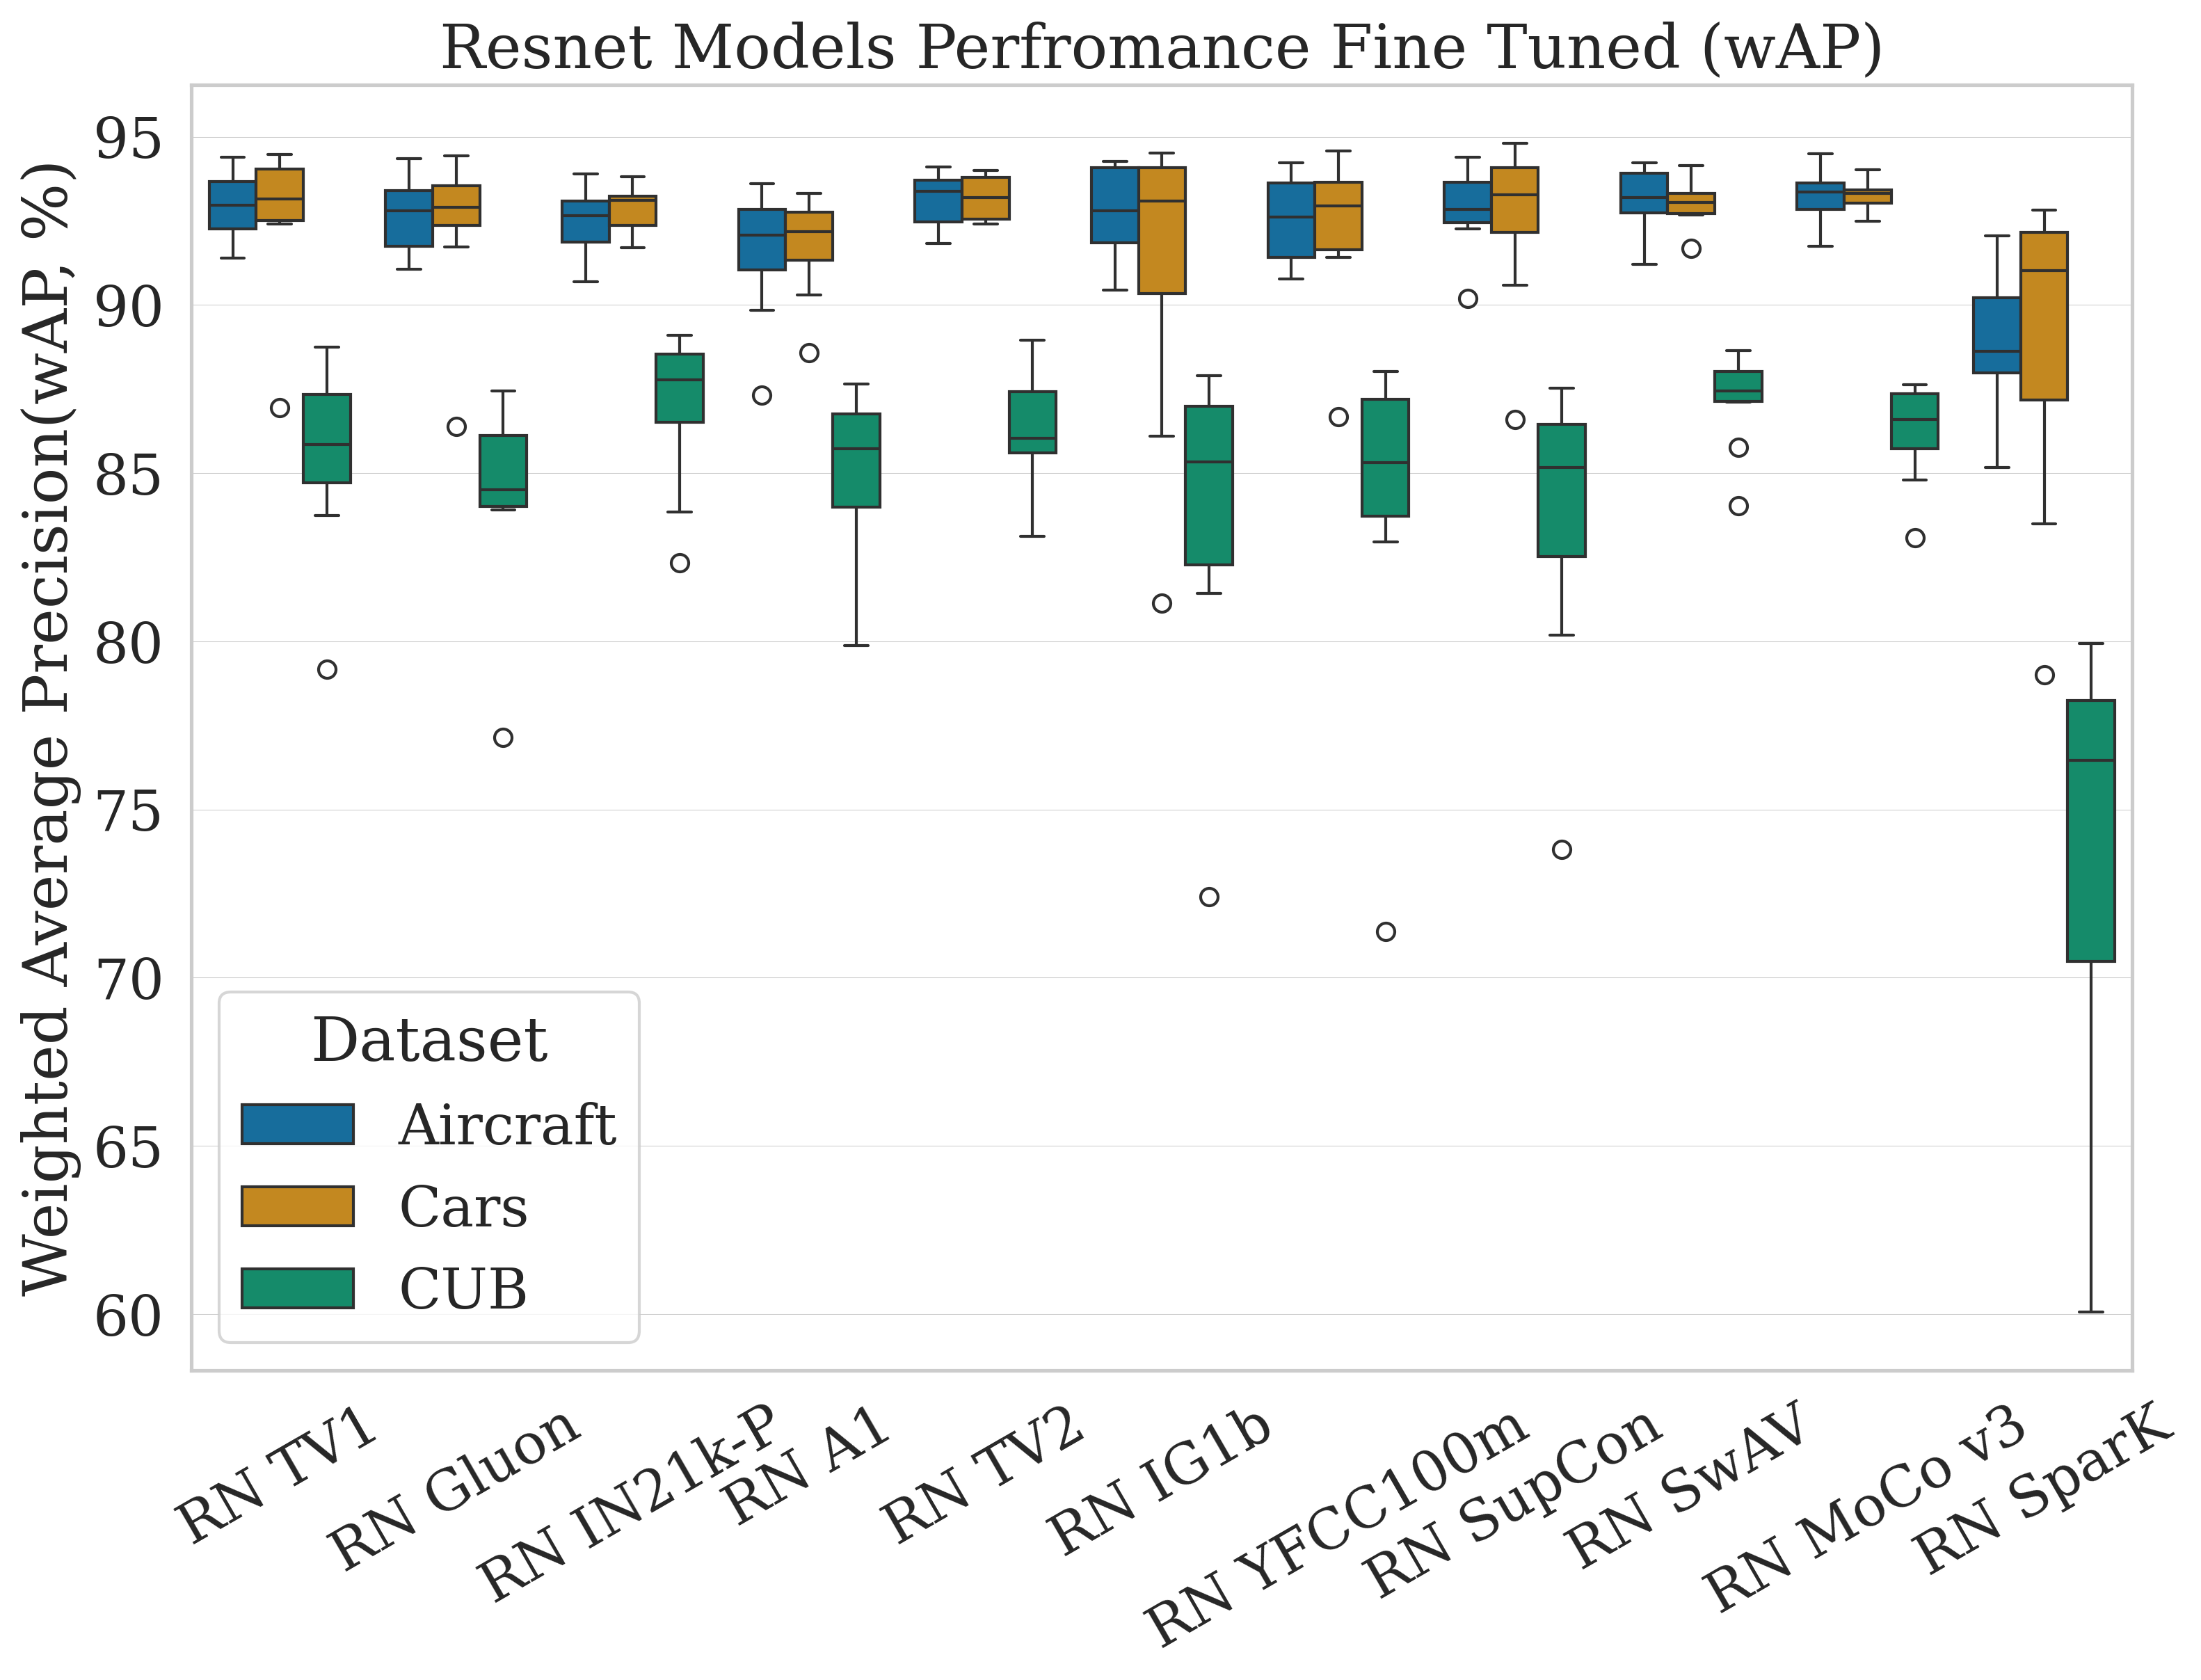
\includegraphics[width=\linewidth]{figures/imgs/rn_ft.png}
        \label{fig_rn_ft}
    \end{minipage}
    \hspace{0.01\linewidth} 
    \begin{minipage}{0.43\linewidth}
        \centering
        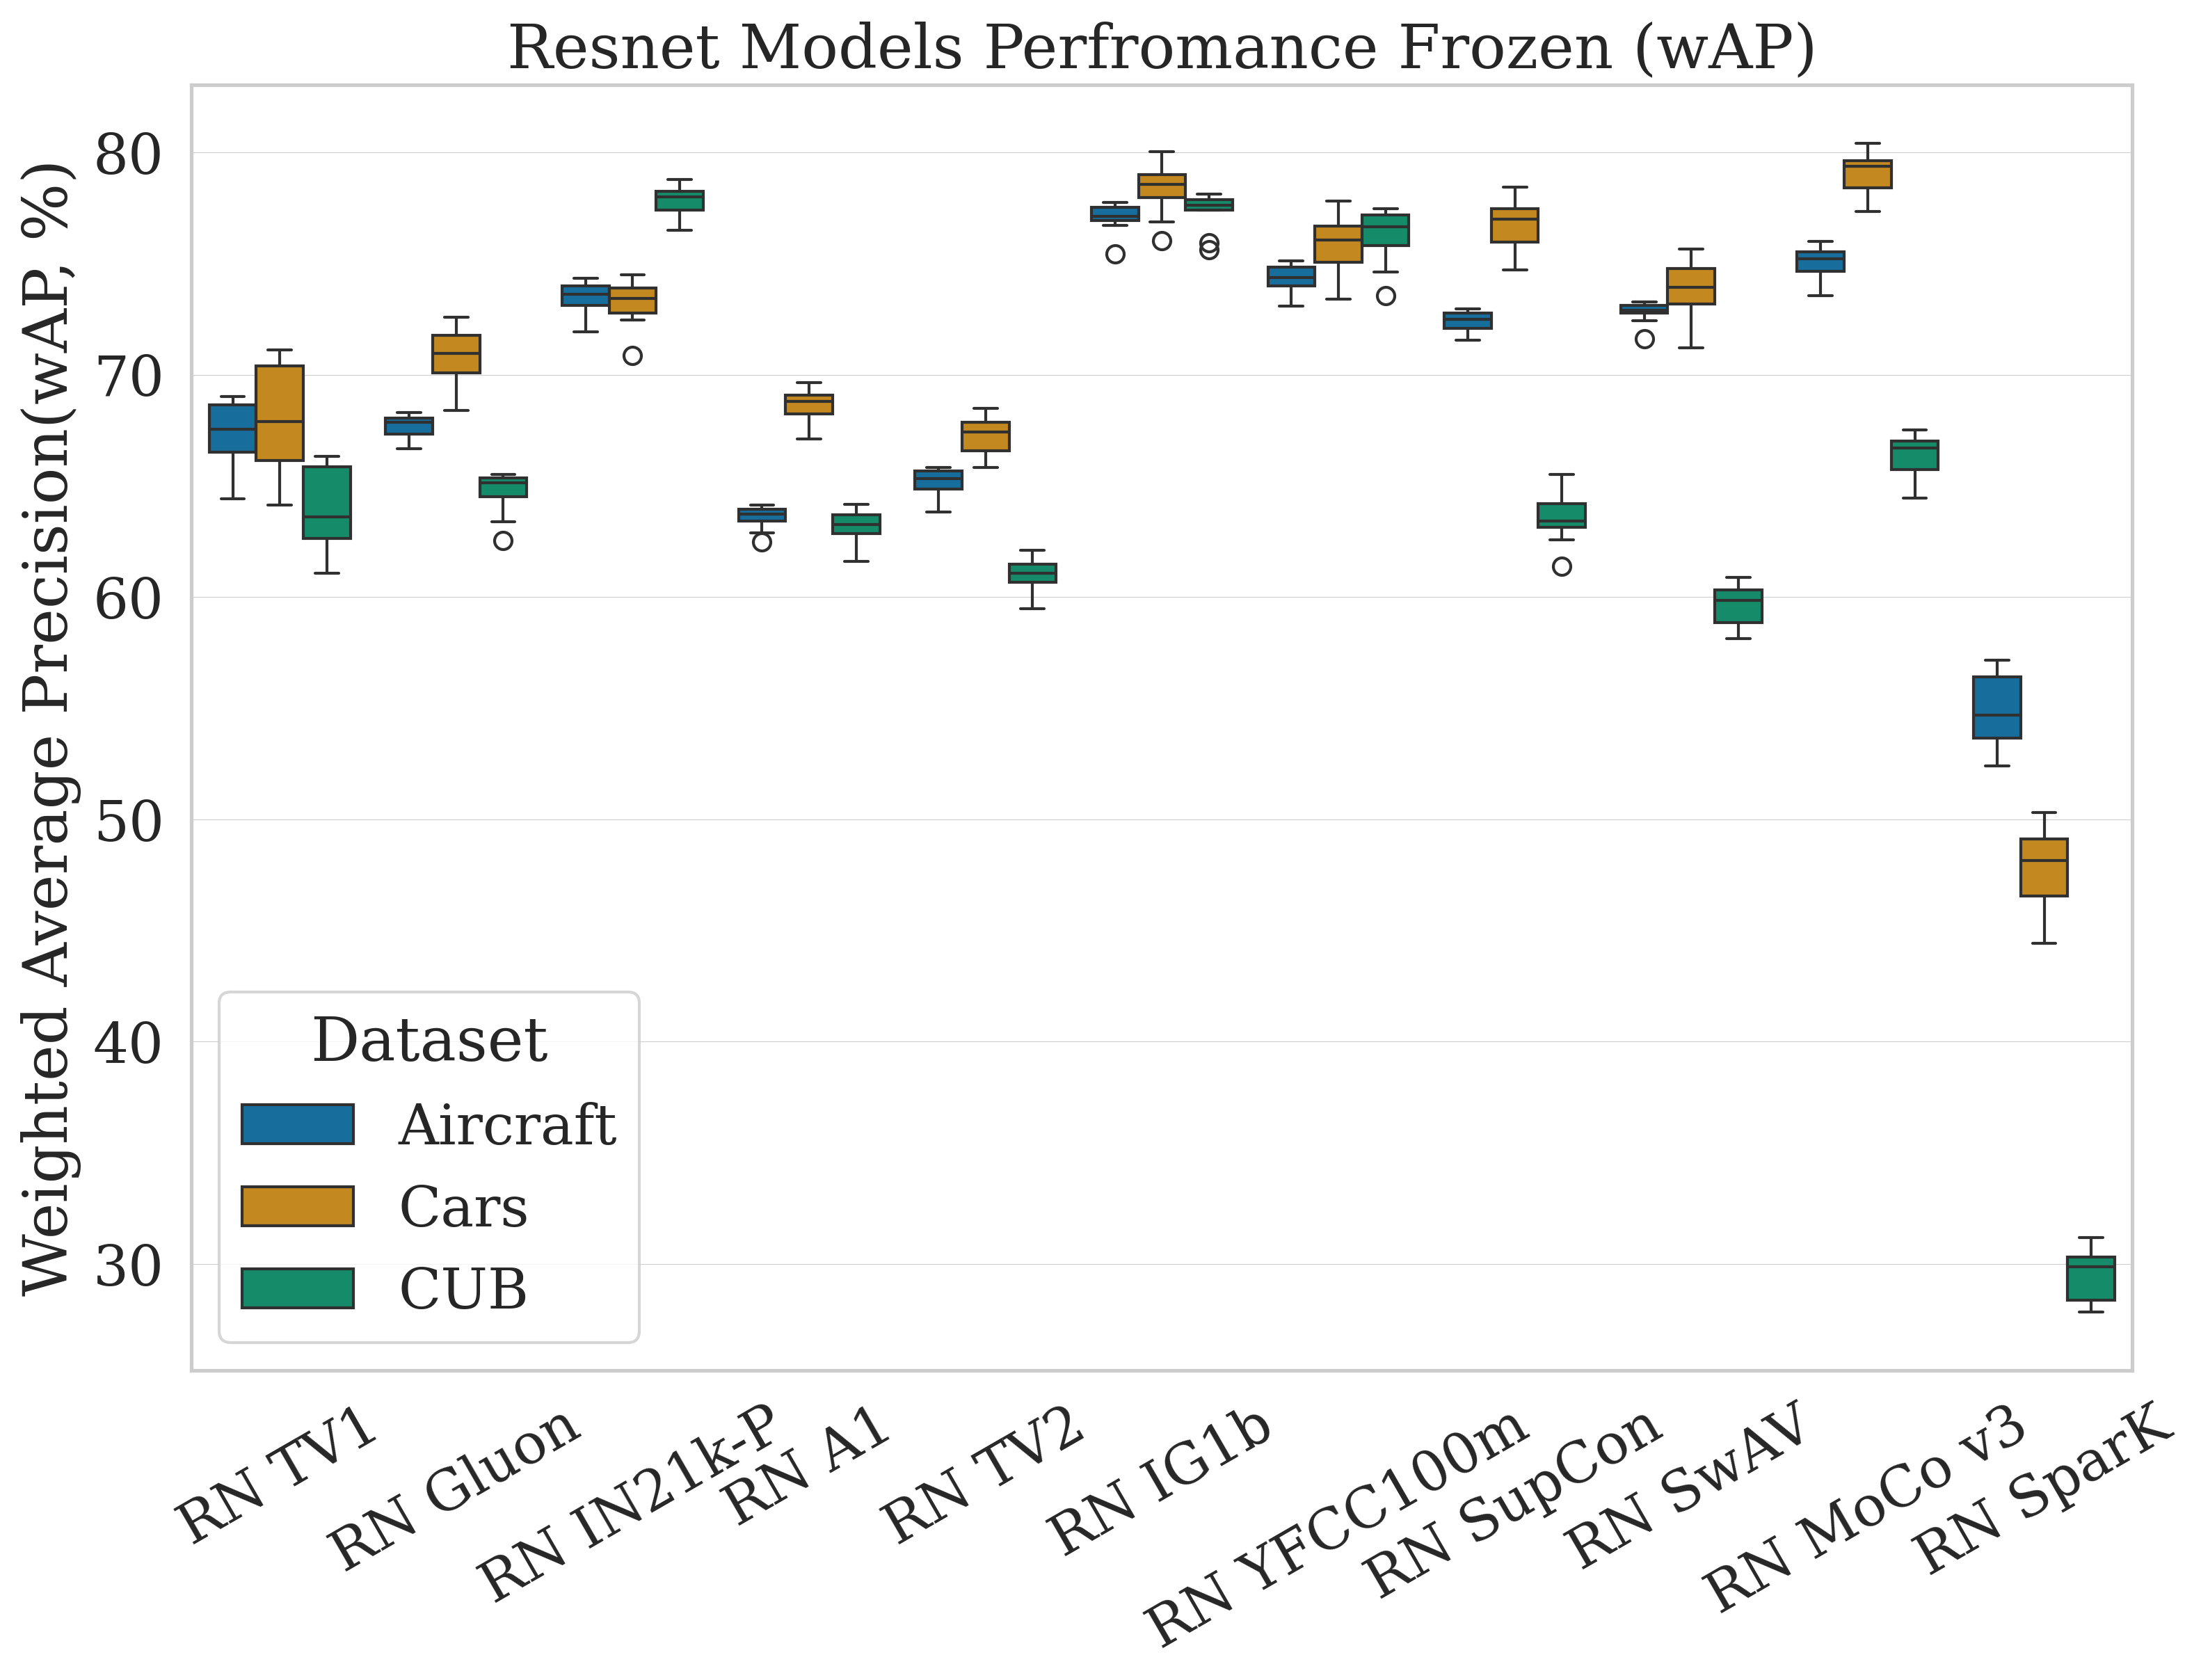
\includegraphics[width=\linewidth]{figures/imgs/rn_fz.png}
        \label{fig_rn_fz}
    \end{minipage}

    \centering
    \begin{minipage}{0.43\linewidth}
        \centering
        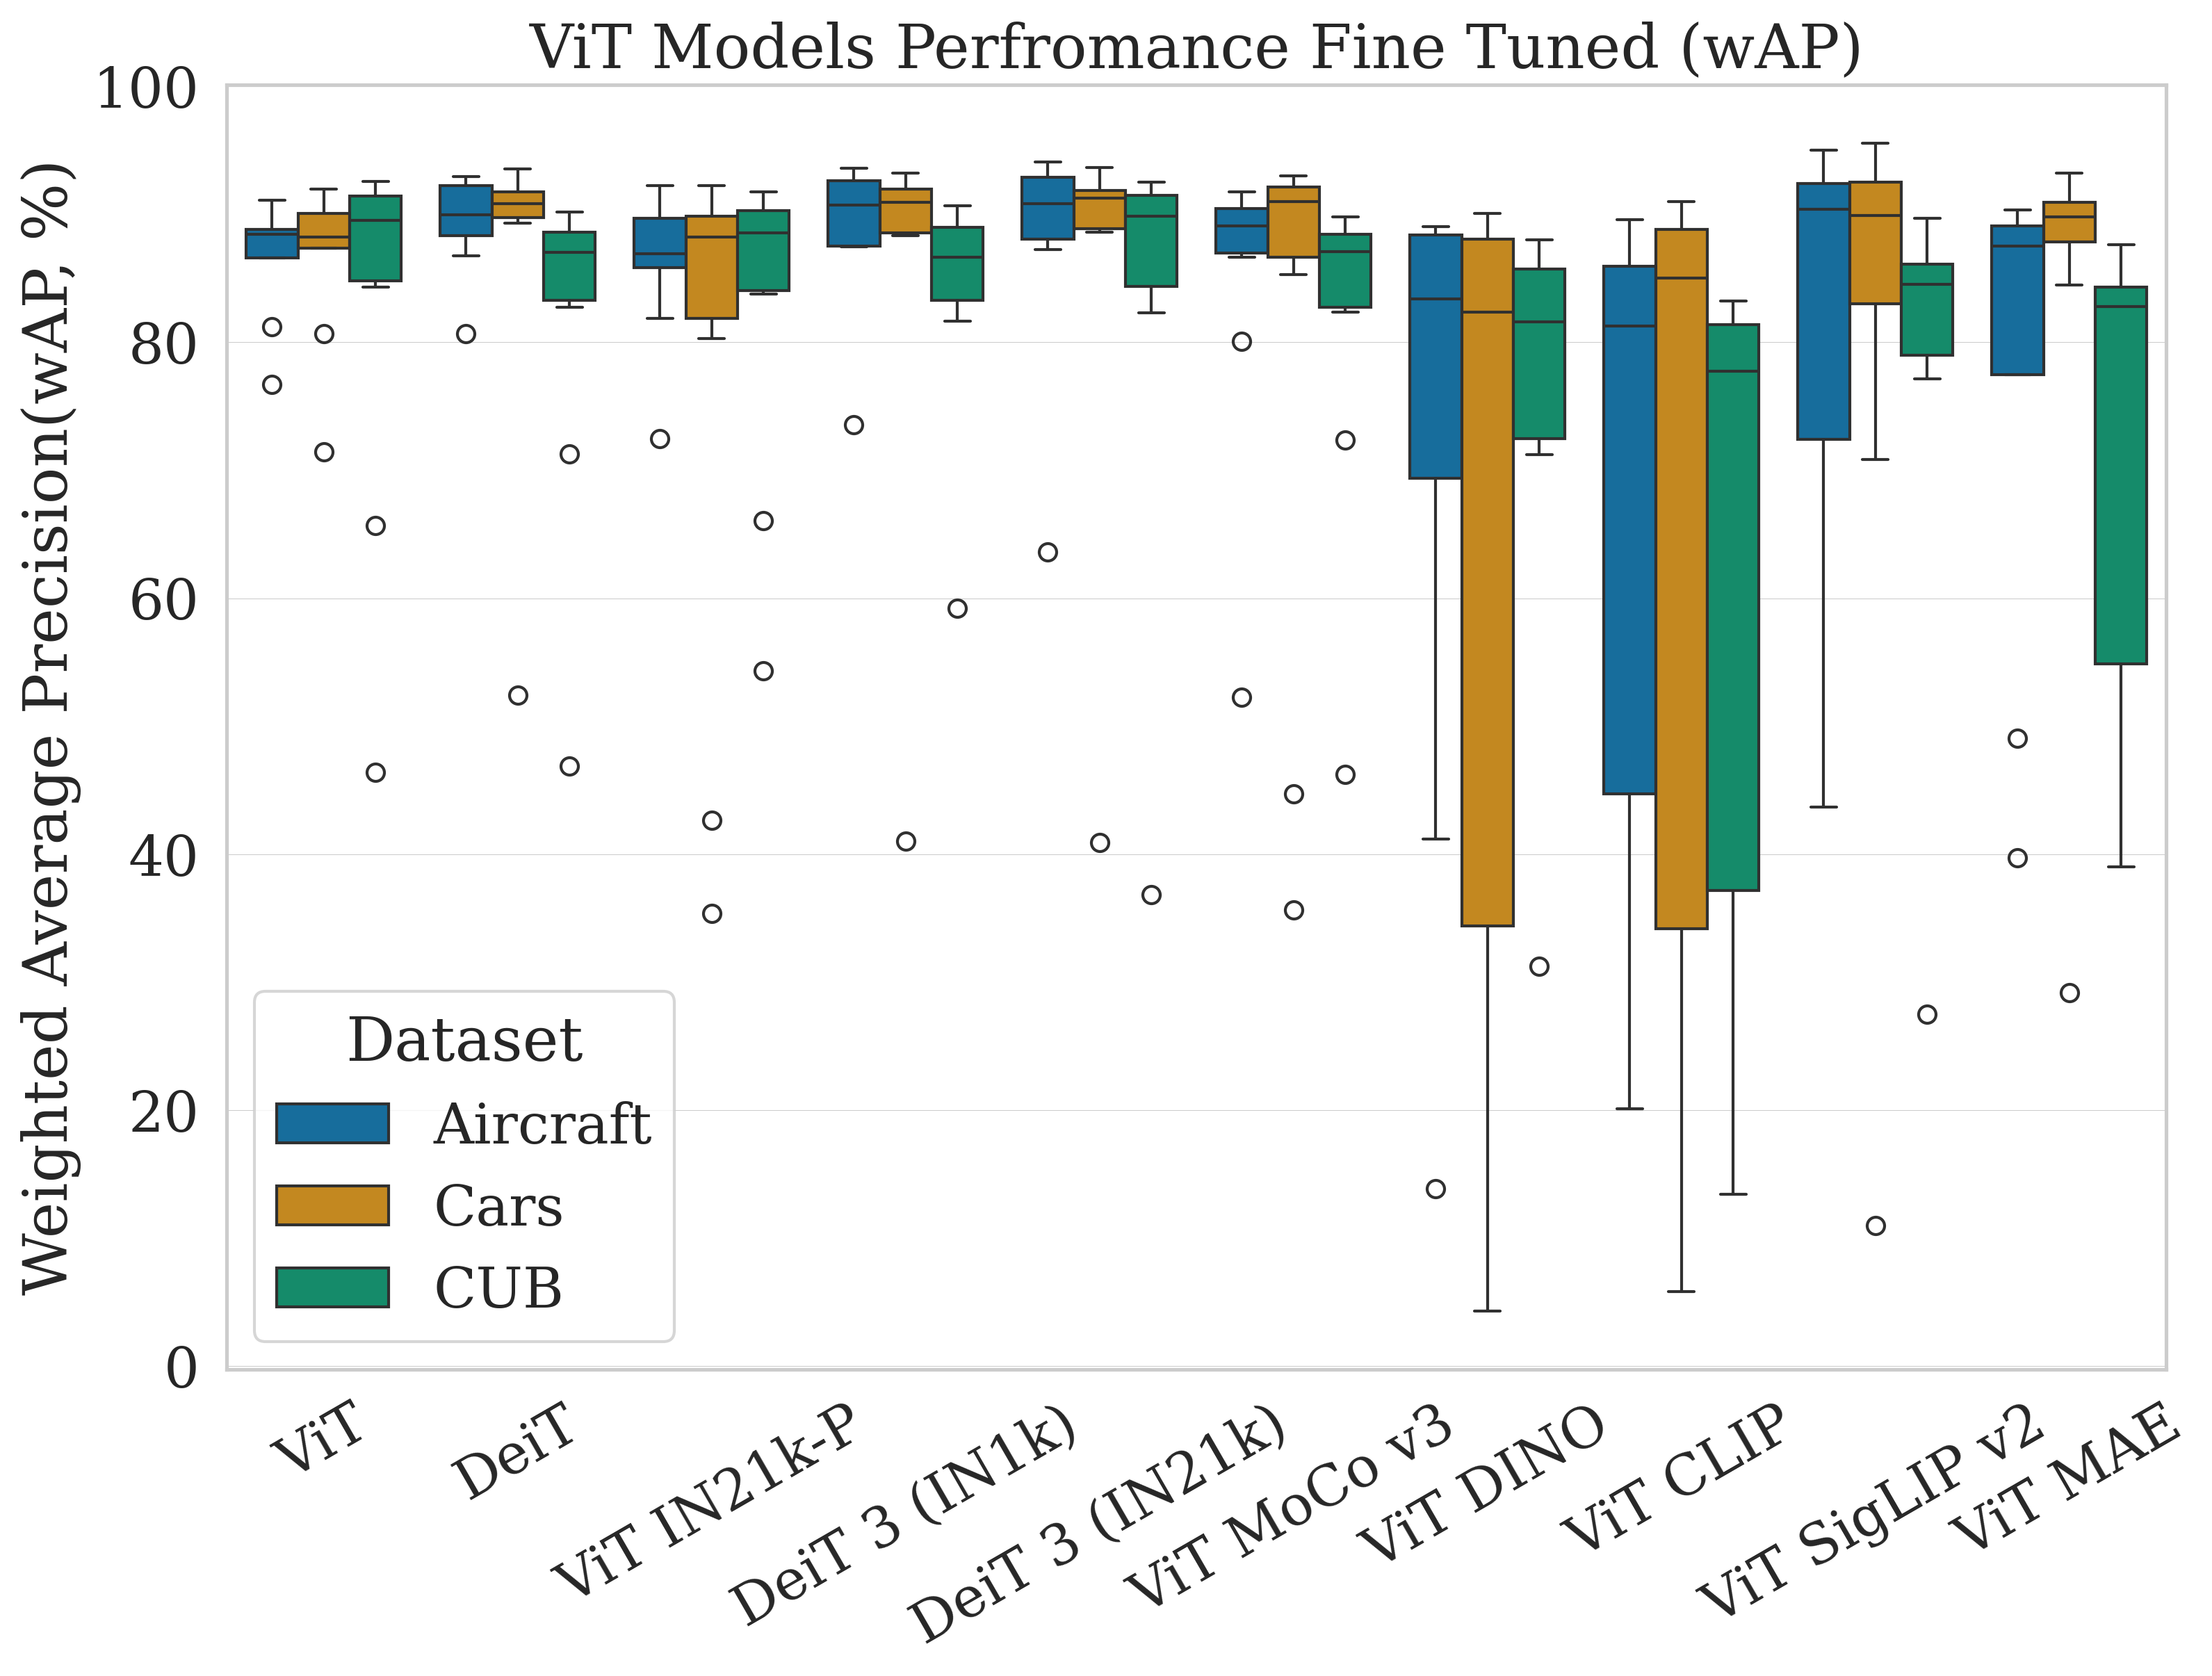
\includegraphics[width=\linewidth]{figures/imgs/vit_ft.png}
        \label{fig_vit_ft}
    \end{minipage}
    \hspace{0.01\linewidth} 
    \begin{minipage}{0.43\linewidth}
        \centering
        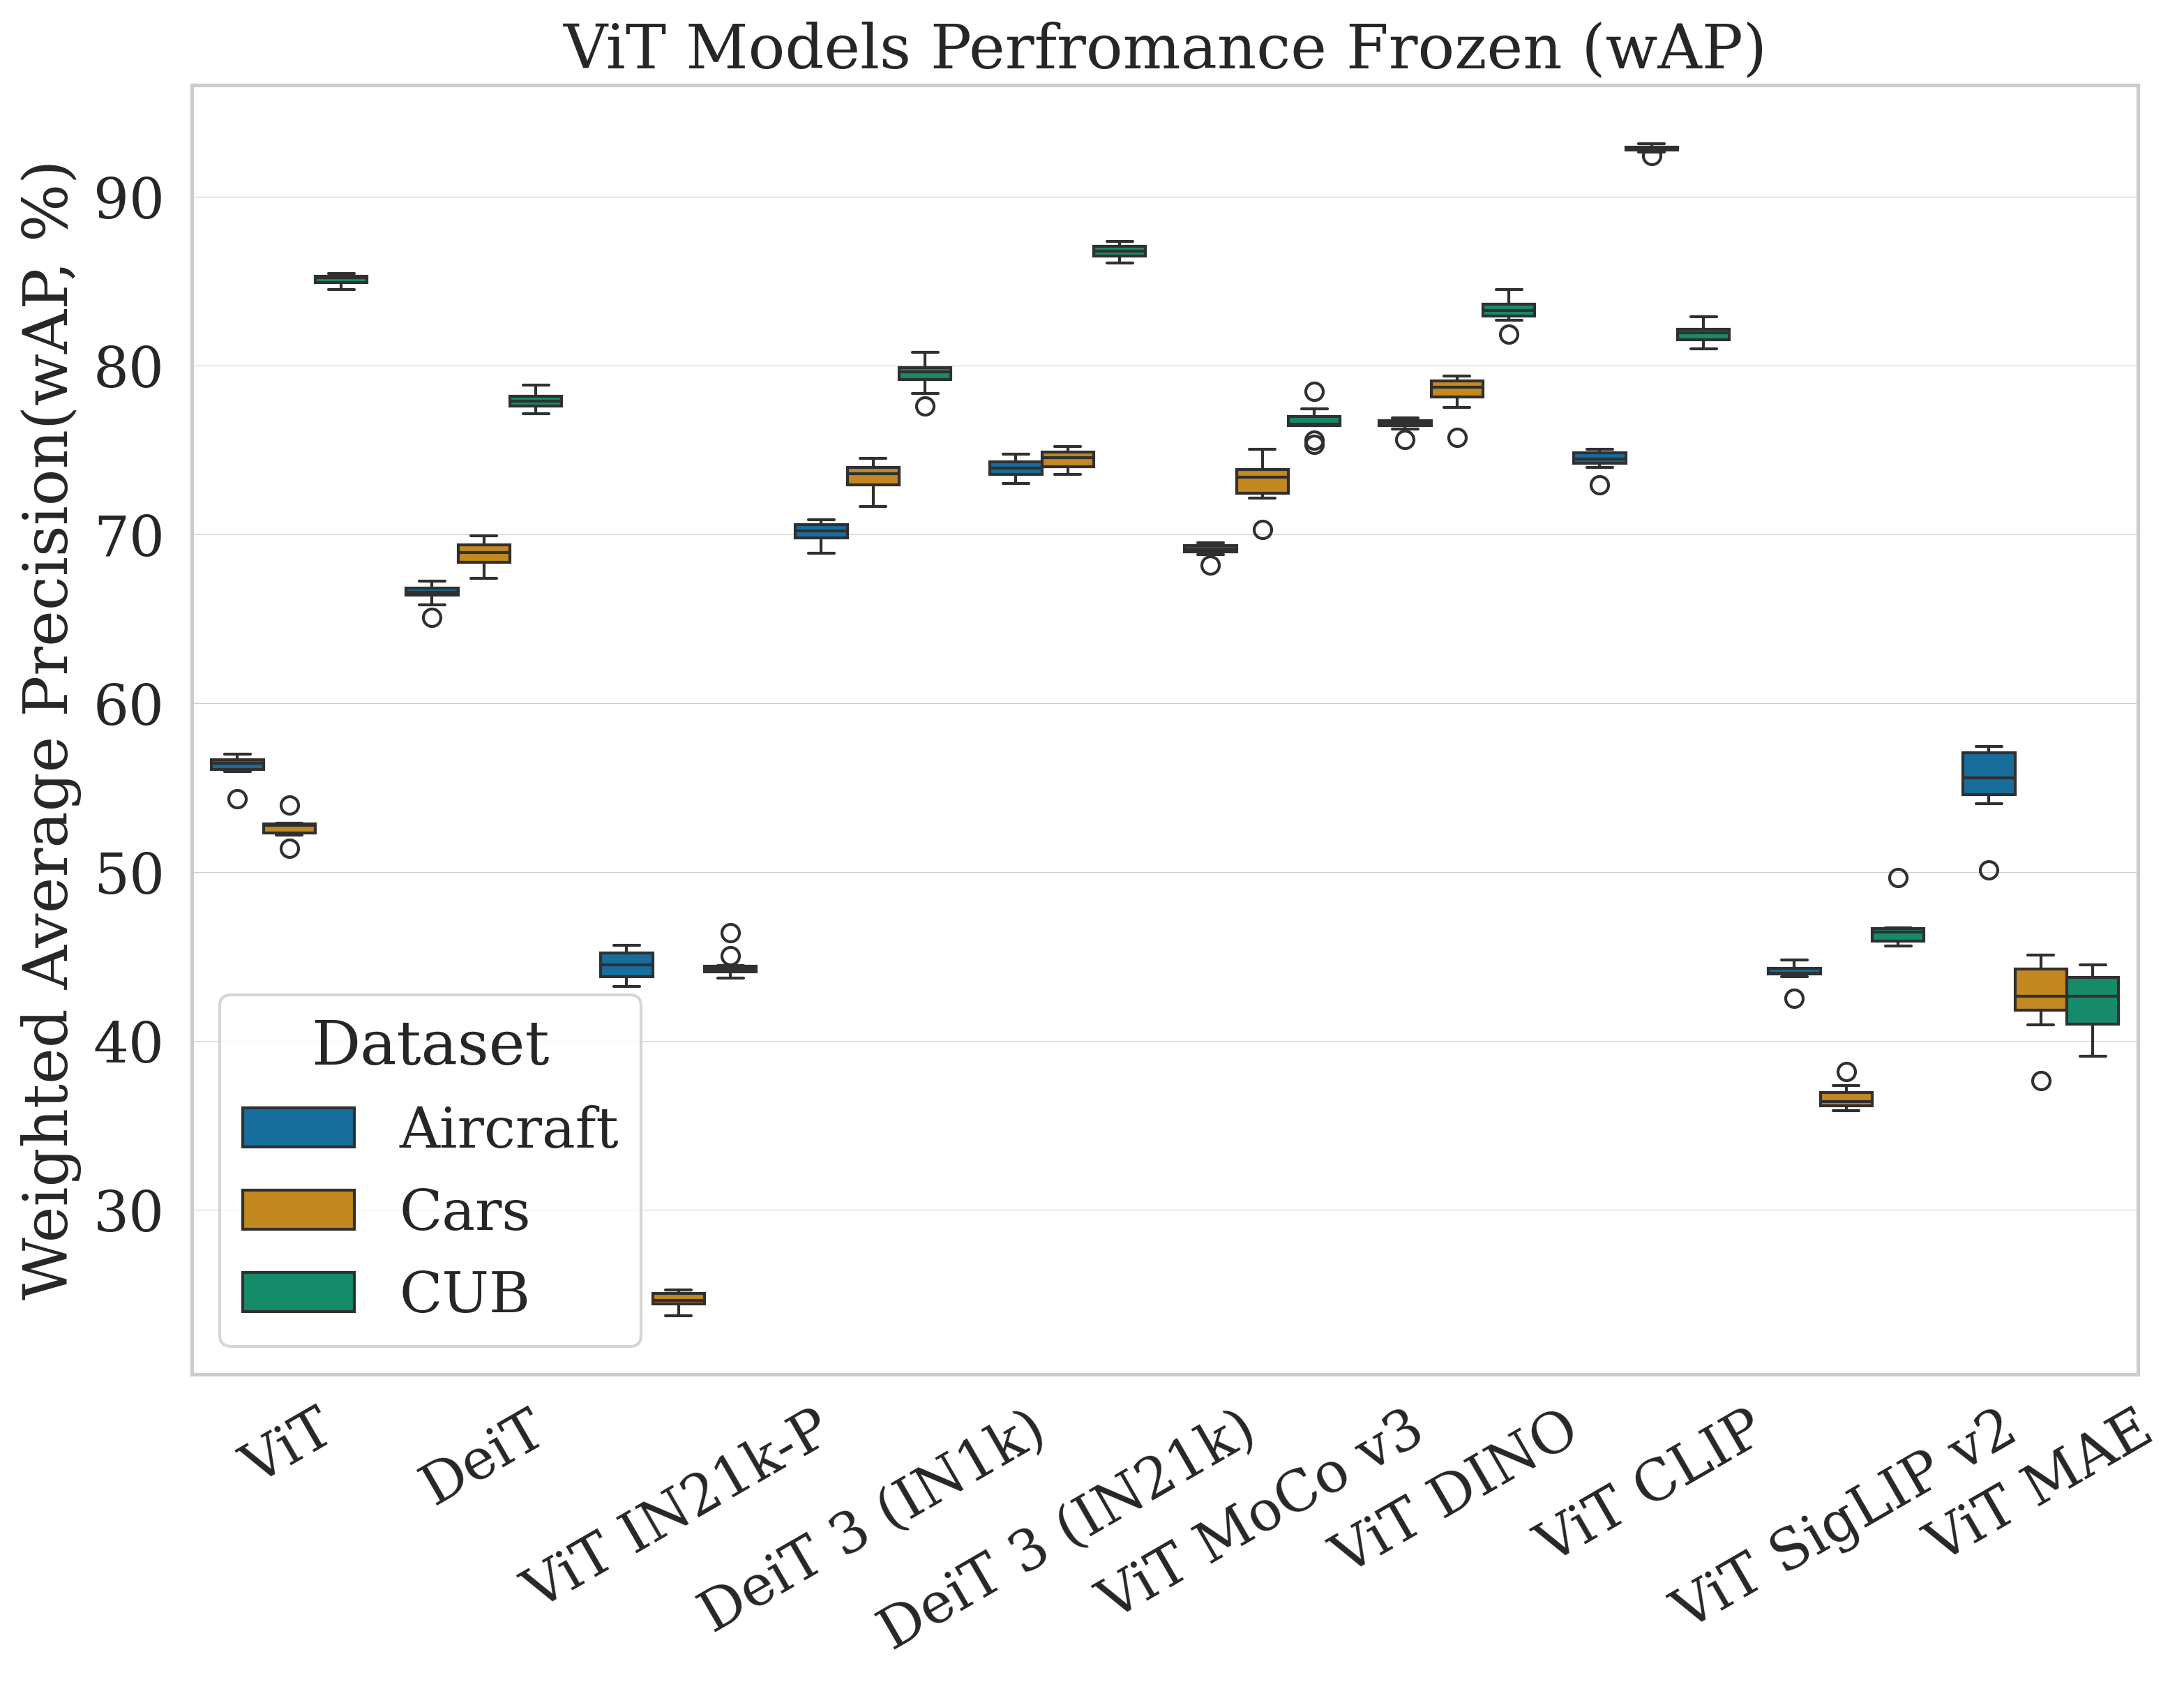
\includegraphics[width=\linewidth]{figures/imgs/vit_fz.png}
        \label{fig_vit_fz}
    \end{minipage}
    \vspace{-0.55cm}
    \caption{Backbone performance across training regimes. We compare ResNet (top) and ViT (bottom) models under fine-tuned (FT, left) and frozen (FZ, right) settings. Each plot shows the wAP performance distribution across models with different pretraining strategies.}
    \label{fig_four_plot}
\end{figure*}

\subsection{Impact of introducing Hierarchy on FGIR}

\begin{table}[t]
\centering
\caption{ADA ratio across hyperparameters using RN IG1b as the evaluation backbone. Pseudo-hierarchies are constructed with two levels using either the same backbone (RN IG1b) or a stronger backbone (ViT SigLIP v2), with different coarse-label ratios. Lower is better.}
\label{tab:baseline_vs_pseudohierarchy}
\begin{tabularx}{\linewidth}{p{1.8615cm}XXXX}
\toprule
\multirow{2}{*}{Ratio (\%)} 
& \multicolumn{2}{c}{Aircraft} 
& \multicolumn{2}{c}{CUB} \\
\cmidrule(lr){2-3} \cmidrule(lr){4-5}
& IG1b
& SigLiPv2
& IG1b
& SigLiPv2 \\
\midrule
No Hierarchy 
& \multicolumn{2}{c}{3.08} 
& \multicolumn{2}{c}{8.67} \\
\midrule
10 & 1.77 & \underline{1.81} & \underline{7.25} & 9.34 \\
20 & 2.27 & \textbf{1.75} & 8.04 & 8.66 \\
30 & 1.71 & 1.82 & 7.32 & 7.43 \\
40 & 1.77 & 2.43 & \textbf{6.97} & 8.22 \\
50 & \underline{1.68} & 2.08 & 8.02 & \textbf{6.84} \\
70 & \textbf{1.54} & 1.92 & 8.59 & \underline{7.03} \\
\bottomrule
\end{tabularx}
\end{table}

\subsubsection{Introducing hierarchy improves robustness}
Table \ref{tab:baseline_vs_hierarchy} shows that hierarchical supervision consistently improves robustness across architectures, as indicated by lower ADA ratios compared to baseline. In ResNet models, hierarchy can reduce ADA ratio by almost half. For example, ResNet IG1b on Aircraft decreases from 3.079 to 1.729. This effect is more pronounced for ViT models, which are more sensitive to hyperparameter choices. ViT base on Aircraft drops ADA by nearly fourfold from 24.997 to 6.250.

\subsubsection{Hierarchy is more effective on machine-centric datasets}
The impact of hierarchical supervision varies across datasets, with larger ADA reductions observed on Aircraft and Cars as shown in Table \ref{tab:baseline_vs_hierarchy}. For example, ResNet IG1b sees ADA decrease from 3.079 to 1.729 on Aircraft and from 6.691 to 0.698 on Cars, whereas on CUB the reduction is smaller, from 7.035 to 6.191. This trend may reflect dataset-specific characteristics discussed in our backbone analysis \ref{sec:dataset_differences}, where more static shapes in Aircraft and Cars compared to more dynamic shapes in CUB, could influence the effectiveness of hierarchy in improving robustness.

\subsection{Pseudo-hierarchy on FGIR}
\subsubsection{Pseudo-hierarchies have a similar effect to human-annotated hierarchies}
As shown in Table \ref{tab:baseline_vs_pseudohierarchy}, ADA ratios for all tested label ratios, constructed using either ResNet or ViT features, are consistently lower than the baseline for both Aircraft and CUB datasets. This proves that hierarchical structure, even when systematically constructed using the proposed BPH algorithm, can improve model robustness across hyperparameters. Pseudo-hierarchies can potentially reduce the ADA ratio by up to half, for example, on the Aircraft dataset the ResNet IG1b decreases the ADA ratio from 3.08 (baseline without hierarchical labels) to 1.54 when using pseudo-hierarchies at 70\% fine-level labels. These pseudo-hierarchies provide a practical approach to hierarchical supervision without incurring the cost of human labeling.

While the relationship of ADA ratios an pseudo-hierarchy ratios is non-monotonic and depends on the specific experiment settings, 40\%-70\% ratios generally yield stronger robustness improvements across the evaluated settings.

% \subsubsection{Relation of Pseudo-Hierarchy Ratios to Robustness}
% From Table \ref{tab:baseline_vs_pseudohierarchy}, the relationship of ADA ratios and pseudo-hierarchy ratios is \textbf{non-monotonic}, i.e. increasing or decreasing pseudo-hierarchy ratio does not always lead to an increase or decrease of ADA ratio. This implies that the robustness gain comes from the introduction of hierarchical bias itself, rather than from a linear scaling of hierarchical strength. Despite these variability, 40\%-70\% ratios generally yield stronger robustness improvements across the evaluated settings.

\section{Conclusion}
The \textbf{choice of backbone} plays a \textbf{critical role} in hierarchical FGIR. By revisiting the pipeline of Chang et al. \cite{chang_your_2021} with \textbf{systematic backbone and hyperparameter selection}, we achieve \textbf{state-of-the-art results}, even with \textbf{older architectures}. Our findings further underscore that \textbf{hyperparameter tuning exerts a substantial influence} on model performance, with \textbf{ResNet models more robust than ViTs} regardless of hyperparameters. In particular, \textbf{discriminative models} (e.g., MoCoV3, SwAV) yield strong performance with both \textbf{high accuracy and low deviation}. The ADA ratio highlights the performance of models with hyperparameter choices in mind and offers a consistent basis for comparing architectures. Beyond backbone selection, hierarchical supervision improves robustness, and pseudo-hierarchies constructed from feature representations provide similar gains to human-annotated hierarchies, showing that the benefits arise from the hierarchical inductive bias itself rather than from manual label design. This makes pseudo-hierarchy construction as an effective and scalable alternative that can reduce annotation cost, and future work could explore methods to evaluate pseudo-hierarchy quality without full hierarchical FGIR training.

% As such, it serves as a useful metric for guiding model selection for future hierarchical FGIR research. Our observation shows the need for new transferability metrics that account for the hierarchical structure of labels.


\bibliographystyle{IEEEbib}
\bibliography{icme2026references}

\end{document}
